
\section{Perspectives of Optimizing Matching Operator}
In this section, we focus specifically on handling the matching operator, which plays a distinct role
within the \spjm queries compared to the \spj queries. We discuss two main perspectives of optimizing
the matching operator: logical transformation and physical implementation. Logical transformation is
responsible for transforming a matching operator into a logically equivalent representation for further solving,
while physical implementation focuses on how the matching operator can be efficiently executed.

\subsection{Logical Transformation}
\label{sec:handling-match-operator}
We commence with an intuitive, graph-agnostic method before
introducing a graph-aware technique grounded on the concept of decomposition tree, which
is the key to the optimization of graph pattern matching in the literature~\cite{huge,GLogS}.

Before proceeding, we introduce the concept of pattern decomposition that decomposes $\pattern$ into two overlapping patterns, $\pattern_1$ and $\pattern_2$, with shared vertices $V_{o} = V_{\pattern_1} \cap V_{\pattern_2}$ and shared edges $E_{o} = E_{\pattern_1} \cap E_{\pattern_2}$.
Denote $\pattern = \pattern_1 \cup \pattern_2$. Under the homomorphism semantics, the matching of $\pattern$ can be represented as:

\begin{equation}
    \label{eq:join-pattern}
    \matching(\pattern) = \matching(\pattern_1) \widehat{\Join}_{V_{o}, E_{o}} \matching(\pattern_2),
\end{equation}
where $\widehat{\Join}$ is a natural join operator for joining two graph relations based on the common vertices and edges.

It is important to note that \refeq{join-pattern} is also applicable to alternative semantics, including isomorphism and non-repeated-edge~\cite{angles2017foundations}. To support these semantics, a special all-distinct operator can be applied as a filter to remove results that contain duplicate vertices and/or edges. The adoption of the all-distinct operator is compatible with all techniques in this paper.

%There are already a considerable number of research findings and solutions for the SPJ problem \cite{}.
%Given that the main difference between SPJM and SPJ lies in the matching operator, in addressing the SPJM problem, solutions from the SPJ problem can be referenced.
%In this section, we focus on the method to deal with the matching operators.
%Firstly, an intuitive method is presented and then an advanced method based on matching decomposition is proposed.
%For simplicity, the pattern graph given in matching operators are assumed to be connected in this section.

\subsubsection{Graph-agnostic Method}
\label{sec:intuitive-method}
Graph-agnostic methods~\cite{apache-age,DuckPGQ,DuckPGQ-VLDB} (\todo{add more references}) simply recast graph match operations
as a sequence of relational operations (mainly joins and projections). This allows an \spjm query to be naively transformed into an \spj query, which then can be optimized through standard relational optimizers.

Consider a pattern graph $\pattern$ and one of its edges $e = (u_s, u_t)$. According to the definition of the matching operator (\refsec{matching-operator}), the graph edges and vertices that can be matched with $e$ must have the labels $\lab(e)$, $\lab(u_s)$, and $\lab(u_t)$. We further denote the relations corresponding to these edges and vertices via \rgmapping as $R_{\lab(e)}$, $R_{\lab(u_s)}$, and $R_{\lab(u_t)}$, respectively. Moreover, there must be total functions $\lambda_{\lab(e)}^s$ and $\lambda_{\lab(e)}^t$ for mapping tuples from $R_{\lab(e)}$ to $R_{\lab(u_s)}$ and $R_{\lab(u_t)}$, respectively. We define the following EV-join operation regarding $\lambda_{\lab(e)}^s$ as:

\begin{equation} \label{eq:ev-join}
\begin{split}
R_{\lab(e)} & \evjoin R_{\lab(u_s)} = \\
& \{(t_e, t_s) | t_e \in R_{\lab(e)} \land t_s \in R_{\lab(u_s)} \land \lambda_{\lab(e)}^s(t_e) = t_s\}.
\end{split}
\end{equation}

The EV-join regarding $\lambda_{\lab(e)}^t$ is defined analogously. Note that the EV-join is associative, meaning that the order of the edge and vertex relations is not important.


%Such a transformation, as indicated by the following lemma, maintains the integrity of the data and relationships, ensuring a lossless conversion process.
The following lemma shows that there exists a logically equivalent transformation from an \spjm query to an \spj query.

\begin{lemma}
    \label{lem:spjm-to-spj}
    With \rgmapping, an \spjm query given in \refeq{spjm} can be losslessly converted to an \spj query.
\end{lemma}
\begin{proof}
    It suffices to convert the matching operator in \refeq{spjm} into a sequence of relational operators. Consider a pattern $\pattern_m$ of $m$ edges, where the $i$-th vertex is denoted as $u_i$, and the $i$-th edge is $e_i = (u_{s_i}, u_{t_i})$. %According to the $\rgmapping$, the corresponding relations of vertex $u_i$ and edge $e_i$ are denoted as $\relation{u_i}$ and $\relation{e_i}$, respectively. Furthermore, we have $\lambda_{e_i}^s$ and $\lambda_{e_i}^t$ to map tuples from $\relation{e_i}$ to $\relation{u_{s_i}}$, and from $\relation{e_i}$ to $\relation{u_{t_i}}$, respectively.

The proof proceeds by induction, starting with a pattern graph $\pattern_0$ with a single vertex and no edges. It is clear that $\matching(\pattern_0)$ yields a subset of vertices with label $l_{u_0}$, which is mapped from the relation $\relation{u}$ via $\rgmapping$. As a result, we have $R_0 = \gproject(\matching(\pattern_0)) = \relation{\lab(u_0)}$.

Next, consider $\pattern_1$ with one edge, $e_1 = (u_{s_1}, u_{t_1})$. Matching $\pattern_1$ is equivalent to retrieving the edge relation, together with the corresponding source and target vertices. Therefore, we have:
\[ R_1 = \gproject(M(\pattern_1)) = \relation{\lab(u_{s_1})} \evjoin \relation{\lab(e_1)} \evjoin \relation{\lab(u_{t_1})} \]

Assume that when $m = k-1$, $\gproject(\matching(\pattern_{k-1}))$ can be losslessly converted to a sequence of relational operators, resulting in the relation $R_{k-1}$. When $m = k$, we consider $\pattern_{k}$ of $k$ edges that is constructed from $\pattern_{k-1}$ by adding one more edge $e_k = (u_{s_k}, u_{t_k})$. For $\pattern_{k}$ to be connected, it must share at least one common vertex $V_o$ with $\pattern_{k-1}$. According to \refeq{join-pattern}, we have:
\[ \matching(\pattern_{k}) =  \matching(\pattern_{e_k}) \gjoin_{V_o} \matching(\pattern_{k-1}), \]
where $\pattern_{e_k}$ denotes a pattern that contains only the edge $e_k$, and $V_o$ is the common vertex shared by $\pattern_{k-1}$ and $\pattern_{e_k}$. Applying $\gproject$ to the above equation, we get:
\begin{equation*}
\begin{split}
R_k &= \gproject(\matching(\pattern_{k})) \\
    &= \gproject(\matching(\pattern_{e_k})) \Join_{attr_{V_o}}  \gproject(\matching(\pattern_{k-1})) \\
    &= \relation{\lab(u_{s_k})} \evjoin \relation{\lab(e_k)} \evjoin \relation{\lab(u_{t_k})} \Join_{attr_{V_o}} R_{k-1}
\end{split}
\end{equation*}
By induction, denoting $R'_i = \relation{\lab(u_{s_i})} \evjoin \relation{\lab(e_i)} \evjoin \relation{\lab(u_{t_i})}$, we have the matching operator losslessly converted to a sequence of relational operators:
\begin{equation}
    \label{eq:graph-agnostic}
    \gproject(\matching(\pattern_{k})) = R'_k \Join R'_{k-1} \Join \cdots \Join R'_1 \Join R_0.
\end{equation}

We thus conclude the proof.
\end{proof}

\comment{
Some existing works have adopted this idea and implemented translators to convert SPJM queries to SPJ queries.
Two typical products include Apache Age \cite{apache-age} and DuckPGQ \cite{DuckPGQ,DuckPGQ-VLDB}.
}

\begin{example}
    Given pattern graph $\pattern$ shown in \reffig{intro-rgmapping-example}(b), the matching operator $\matching(\pattern)$ can be converted to a sequence of relational operators as follows.

    Without loss of generality, we start from $\pattern_0$ with only $u_{p_1}$, and we have $\relation{0} = \relation{\text{Person}}$.
    Next, $e_1 = (u_{p_1}, u_{p_2})$, $e_2 = (u_{p_1}, u_m)$, and $e_3 = (u_{p_2}, u_m)$ are sequentially added into $\pattern_0$ , and we have
    \begin{equation*}
      \begin{split}
        R'_1 = \relation{\text{Person}} \Join_{person\_id=pid1} \relation{\text{Knows}} \Join_{pid2=person\_id} \relation{\text{Person}}, \\
        R'_2 = \relation{\text{Person}} \Join_{person\_id=pid} \relation{\text{Likes}} \Join_{mid=message\_id} \relation{\text{Message}}, \\
        R'_3 = \relation{\text{Person}} \Join_{person\_id=pid} \relation{\text{Likes}} \Join_{mid=message\_id} \relation{\text{Message}}.
      \end{split}
    \end{equation*}
    \todo{Must refine the cases of Person1 and Person2, which may not be correct.}
    We finally have $\gproject(\matching(\pattern)) = R_0 \Join R'_1 \Join R'_2 \Join R'_3$.


    %For the SPJM query shown in Fig.~\ref{fig:spjm}, it can be transformed to the SPJ query as follows:
    %\begin{equation*}
    %    \pi_A(\sigma_d(\pi_{A'}(Person \Join Likes \Join Message \Join Likes \Join Person) \Join Place))
    %\end{equation*}
    %Then, this SPJ query can be optimized with relational optimizers.
\end{example}

Given that edges may connect to common vertices, it becomes apparent that there are some redundant joins in \refeq{graph-agnostic}. Removing these redundancies results in a sequence of joins corresponding to the number of vertices and edges in the pattern graph, as illustrated in the above example.

\subsubsection{Graph-aware Method}
\label{sec:graph-aware}
The graph-agnostic method, which converts the matching operator into a sequence of relational operators, is straightforward and easy to implement. However, it may be inefficient because relational optimizers treat relations representing vertices and edges equally as the other relations, preventing the optimizer from utilizing graph-specific optimization techniques. %Furthermore, relational optimizers are known to struggle with queries containing a large number of joins, which is a common case in graph pattern matching.

In this section, we introduce a graph-aware method that incorporates key ideas from the literature on graph optimization. Following \refeq{join-pattern}, we can recursively decompose $\pattern$, forming a tree structure called the \emph{decomposition tree}. The tree has a root node that represents $\pattern$, and each non-leaf \emph{intermediate} node is an \emph{induced} sub-pattern (a subgraph of the pattern) $\pattern' \subset \pattern$, which has a left and right child node, denoted as $\pattern'_l$ and $\pattern'_r$, respectively. %The condition of the intermediate pattern being induced
The leaf nodes of the tree are called \emph{Minimum Matching Components} (\mmc), correspond to indivisible patterns directly solvable with specific physical operations
as will be introduced in~\refsec{xx}. The decomposition tree naturally forms a logical plan for solving $\matching(\pattern)$, as demonstrated in \reffig{xx}. For any non-leaf node $\pattern'$, there exists a relationship $\matching(\pattern') = \matching(\pattern'_l) \gjoin \matching(\pattern'_r)$ according to \refeq{join-pattern}. The plan allows for the recursive computation of the entire pattern.

We follow~\cite{huge} to use a single-edge pattern as well as a \emph{complete star} as an \mmc. We denote a star-shaped pattern as $\pattern(u;S)$, where $u$ denotes the root vertex of the star and $S$ is the set of leaf vertices\footnote{The edge directions among $u$ and $S$ are not important, and we assume they  all point from $u$ to $S$.}.
In the decomposition tree, given $\pattern' = \pattern'' \cup \pattern(u;S)$, $\pattern(u;S)$ is called a complete star if and only if it is a right child and $S \subseteq V_{\pattern'}$, indicating that the leaf vertices of the complete star must all be common vertices for the decomposition. The complete star is a logical representation of the physical operations of \expand and \intersection, which are key to the implementation worst-case optimal join algorithm~\cite{mhedhbi2019optimizing} for graph pattern matching, as will be discussed in \refsec{xx}.

\comment{
Therefore, decomposing the matching operators recursively can finally result in a tree, whose leaf nodes are MMCs.
To ensure worst-case optimality, in the process of decomposition, the pattern graph of each decomposed matching operator should be an induced subgraph of $\mathcal{P}_0$.
The generated tree is called a decomposition tree and it is actually a logical plan of the matching operator.
\modify{Without loss of generality, the left-deep join order is employed on the tree.}

Then, it is crucial to identify which matching operators to treat as MMCs.
We adopt the definition of \emph{complete star} from \cite{huge}.
Specifically, suppose $\matching(GR, \mathcal{P})$ is decomposed into $\matching(GR, \mathcal{P}_1)$ $\widehat{\Join}$ $\matching(GR, \mathcal{P}_2)$, $\mathcal{P}_2$ is called a complete star iff $\mathcal{P}_2$ is a star $(v_r; \mathcal{H})$, $\mathcal{H} \subseteq E_{\mathcal{P}_1}$, and $|\mathcal{H}| \geq 2$, where $v_r$ is the root and $\mathcal{H}$ is the set of its leaf vertices.
Inspired by HUGE \cite{huge} and GLogS \cite{GLogS}, matching operators located on the right subtree of the join operator with complete stars as the pattern graphs are the MMCs in this paper.

Besides, a matching operator located on the left subtree of the join operator is an MMC iff its pattern graph is an edge (i.e., one edge and its adjacent two vertices).
}

\begin{figure}
    \centering
    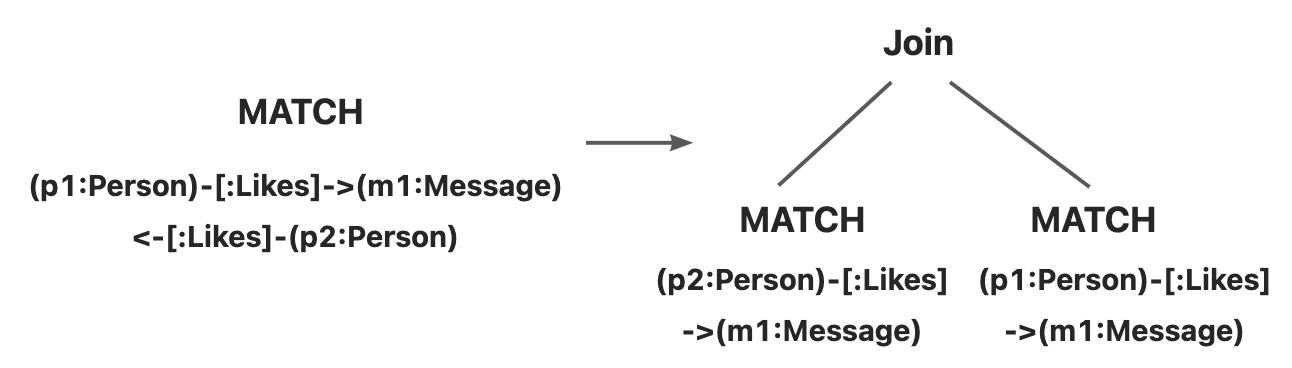
\includegraphics[width=.8\linewidth]{./figures/match-decompose.png}
    \caption{Decomposion of the match operator in the SPJM query shown in Fig.~\ref{fig:spjm}.}
    \label{fig:match-decomposition}
\end{figure}

\begin{example}
    \todo{the sample and figure must all be refined.}
    Given the matching operator in Fig.~\ref{fig:spjm}, it is decomposed into two matching operators as shown in Fig.~\ref{fig:match-decomposition}.
    For the right matching operator, because its pattern is a complete star $(p_1, \{m_1\})$, the operator is an MMC.
    For the left matching operator, as its pattern is an edge pattern, it is also an MMC.
    Therefore, the decomposition tree cannot be further decomposed and is a logical plan.
\end{example}

Upon initial examination, the logical plan generated by the decomposition tree, particularly when all the \mmcs are single-edge patterns,
may appear similar to the graph-agnostic method presented in \refsec{intuitive-method}. However, an essential distinction lies in the fact that the graph-agnostic method consistently decomposes the matching of a single-edge pattern into joins of the corresponding vertex and edge relations, whereas the graph-aware method does not. The issues with the graph-agnostic method are towfold. Firstly, it can lead to increased complexity in query optimization, as will be discussed in the subsequent section. Secondly, it may result in the relational optimizer altering the order of joining vertex and edge relations, thereby overlooking the opportunity to utilize graph indexes for the efficient computation of adjacent edges and vertices, as will be further elaborated upon in \refsec{xx}.

\subsubsection{The Search Space: Graph-agnostic vs Graph-aware}
\label{sec:compare-search-space}

In this section, we demonstrate the superiority of the graph-aware method by theoretically proving that the search space employed by the graph-aware method is significantly smaller than that of the graph-agnostic method for optimizing the matching operator in an \spjm query.
Consider a pattern $\pattern$ consisting of $n$ vertices and $m$ edges.

For the purpose of this analysis, we adopt the volcano optimizer~\cite{columbia} for the graph-agnostic method, which is one of the most widely utilized relational optimizer. The original paper introducing the volcano optimizer~\cite{columbia} provided only an upper bound for the search space. In this work, we contribute to the analysis by deriving a lower bound and comparing it to the upper bound of the graph-aware method, thereby enhancing the constructiveness of the comparison. Although there may exist other relational optimizers~\cite{xx} that exhibit greater efficiency in terms of search space, our study remains sound within a generic context.

For matching the pattern, the graph-agnostic method must produce a sequence of joins among $n$ vertex relations and $m$ edge relations, and then utilize a volcano optimizer to search for the optimal join order. We have the following theorem.

\begin{theorem}
    \label{thm:complexity-of-volcano}
    Given a join among $n + m$ relations, the search space for a volcano optimizer is at least $O(4^{m+n-1})$.
\end{theorem}

\begin{proof}
    \todo{refine the proof.}
    We first construct a graph with these $n + m$ relations.
    Specifically, each relation corresponds to a vertex in this graph, and if there is a join condition w.r.t.~two relations, there is an edge between the corresponding vertices.
    To avoid cross product, everytime two relations are joined together, there should be join conditions between them.
    Therefore, the join order can be represented as a spanning tree in the graph.
    By computing the number of physical plans can be generated according to each spanning tree, the total number of physical plans can be obtained.

    In this proof, we compute the number of physical plans for one spanning tree, and this number is a lower bound of the number of physical plans that can be generated.

    We start with a spanning tree with $k$ edges ($k \geq 1$), which has only one leaf node (i.e., it is a path).
    Then, the number of logical plans corresponding to the spanning tree is
    \begin{equation*}
        \begin{split}
            c_l(k) & = 2 * (c(0)c(k-1) + c(1)c(k-2) + \cdots + c(k-1)c(0)) \\
            & = 2\Sigma_{i=0}^{i=k-1}c(i)c(k-1-i), \\
            & \text{where } c_l(0) = 1.
        \end{split}
    \end{equation*}
    With the generating function, it is obtained that
    \begin{equation*}
        \begin{split}
            c_l(k) & = \frac{2^k}{k+1}C(2k, k) \geq \frac{2^k}{k+1}\frac{2k \times \cdots \times (k+1)}{k \times \cdots \times 1} \\
            & \geq \frac{2^k}{k+1}2^{k-1}(k+1) = \frac{4^k}{2}
        \end{split}
    \end{equation*}

    For any spanning tree $T$ with $k = m + n - 1$ edges, denote the longest path in the tree by $p_1$, and its length is $P_1 = |p_1|$.
    By removing the path (i.e., edges in $p_1$) from $T$, we can obtain a new subgraph $T_1$.
    Similarly, the longest path in $T_1$ that intersects with the already removed paths (i.e., $p_1$) is obtained and denoted by $p_2$, with $P_2 = |p_2|$.
    After that, $p_2$ is removed from $T_1$ and subgraph $T_2$ is obtained.
    For $p_1$ and $p_2$, since they are both paths, the numbers of logical plans corresponding to them are $c_l(P_1)$ and $c_l(P_2)$, respectively.
    Without loss of generality, suppose $p_1$ and $p_2$ intersects at vertex $v_i$, and then, $v_i$ appears in each logical plan corresponding to $p_1$.
    Then, by replacing $v_i$ with the plans corresponding to $p_2$, respectively, $c(p_1 \cup p_2) \geq c_l(P_1)c_l(P_2)$ plans are obtained, where $c(t)$ is the number of logical plans corresponding to tree $t$ and $c(t) = c_l(k)$ when $t$ is a path with $k$ edges.

    As $T$ is a tree, by repeatedly finding and removing the paths as above, all the edges in $T$ are finally removed.
    Let the number of paths removed be $s$, we have
    \begin{equation*}
        \begin{split}
            c(T) & = c(p_1 \cup \cdots \cup p_s) \geq c_l(P_1) \cdots c_l(P_s) \\
            & \geq \frac{4^{P_1 + \cdots + P_s}}{2^s} = \frac{4^{m + n - 1}}{2^s} \geq 2^{m+n-1}.
        \end{split}
    \end{equation*}

    %Thus, the number of logical plans w.r.t.~a spanning tree is
    %\begin{equation*}ƒ
    %    \frac{2^{m+n-1}}{m+n}C(2m+2n-2, m+n-1) \geq \frac{4^{m+n-1}}{m+n}.
    %\end{equation*}


    Thus, the number of physical plans is at least $2^{m+n-1}t^{m+n-1} \geq 4^{m+n-1}$, so is the complexity of join order optimization with Calcite.

    In conclusion, Theorem \refthm{complexity-of-volcano} is correct.
\end{proof}


Subsequently, we analyze the search space of the graph-aware method, which is equivalent to the number of possible decomposition trees given a pattern $\pattern$. Although numerous works have been proposed to optimize graph pattern matching~\cite{huge,GLogS,mhedhbi2019optimizing}, to the best of our knowledge, the complexity of the optimization problem has not been thoroughly analyzed. To address this, we construct a graph $\searchgraph_\pattern(V, E)$ to facilitate the analysis, where the vertex set contains all induced sub-patterns of $\pattern$. An edge exists between a larger\footnote{A pattern is considered larger if it contains more vertices.} sub-pattern $\pattern_1$ and a smaller sub-pattern $\pattern_2$ if it is possible for $\pattern_2$ to be the child of $\pattern_1$ in any decomposition tree. We also denote $V_i \subseteq V$ as the set of sub-patterns that contain exactly $i \leq n$ vertices. It is evident that $V_n = \{\pattern\}$.

Determining the exact number of edges in $\searchgraph_\pattern$ for an arbitrary pattern is non-trivial. However, since we are studying the upper bound, we can consider the worst-case scenario. Given a sub-pattern $\pattern'$ consisting of $i < n$ vertices, the remaining $n-i$ vertices can form at most $\binom{n-i}{2}$ (\todo{refine this number}) sub-patterns, which constrains the maximum number of edges that $\pattern'$ can connect to. With this in mind, we can prove the following theorem:

\begin{theorem} \label{theorem:complexity-of-graph-aware}
The search space for determining the optimal decomposition tree for pattern $\pattern$ is at most $O(3^n)$.
\end{theorem}

\begin{proof}
    \todo{refine the proof.}
    Since the considered patterns are all induced subgraphs in GLogS, the complexity of join order optimization is not related to the number of edges (i.e., $m$).
    Then, the join order optimization problem is reduced to a variant of the shortest path problem, and the complexity is $O(\mathcal{E})$, where $\mathcal{E}$ is the number of edges in GLogue.
    In detail,
    \begin{equation*}
        \begin{split}
            %O(\mathcal{E}) & = C(n, n-1)*(2^{n-1}-1) + C(n, n-2) * (2^{n-2}- 1) \\
            %& + \cdots + C(n, 1) * (2^1 - 1) \\
            O(\mathcal{E}) & = \Sigma_{i=1}^{i=n-1}C(n, i)(2^i - 1) = 3^n - 2^{n+1} +1 < 3^n.
        \end{split}
    \end{equation*}

    In conclusion, Theorem \ref{theorem:complexity-of-glogue} is correct.

\end{proof}

Based on the complexity analysis in Theorem \ref{theorem:complexity-of-calcite} and Theorem \ref{theorem:complexity-of-glogue}, it is found that when there is only a matching operator,
\begin{equation*}
    \begin{split}
        \frac{\text{Complexity of Calcite}}{\text{Complexity of relgo}} & > O(\frac{4^{m+n-1}}{3^n}) = O(4^{m-1}(\frac{4}{3})^n).
    \end{split}
\end{equation*}
Therefore, it suggests that GLogS is exponentially faster than Calcite in optimizing matching operators.
It also illustrates the superiority of the decomposition-based method.

\iffalse
\section{Solutions for SPJM Problem}
Two techniques can be applied to assist in solving the SPJM problem.
Since the inputs of matching operators include a graph relation that can be represented as a property graph and a pattern, this process can be regarded as querying on graphs.
Then, the graph structure can be leveraged to generate better plans.
Moreover, in a graph, vertices and edges do not have to be joined one by one and the results of specific substructures can be obtained more efficienctly.
In this section, we first introduce the concepts of the above techniques, and then present different types of methods for solving the SPJM problem.

\subsection{Graph Structure}

The definition of graph structure is as follows.

\begin{definition}[Graph Structure, abbr.~GS]
    Graph structure refers to the connectivity relationships between vertices and edges within the graph, which can be stored in graph indices in varied data structure such as adjacent lists.
\end{definition}

With graph structure, tables can be joined more efficiently.
For example, when two tables representing persons and friendships respectively are joined together, the rows that can be joined are quickly located using graph indices.
Therefore, when graph indices are available, using join methods that can leverage graph indices is a more efficient choice.

\subsection{Graph Matching Decomposition}

A matching operator can be decomposed into two new matching operators.
By joining the results of the new matching operators, the results of the original matching operator can be obtained.
Decomposing the matching operator recursively can result in a tree, which is called the match scanning plan.
Each tree node represents an operator.
\textbf{Without loss of generality, the left-deep join order is employed on the tree}.
Each internal node represents an operator including the join, selection, and projection operator.
Please note that these operators in the tree always map graph relations to graph relations, because in the matching process, graph elements are the smallest units that operators can manipulate.

For internal nodes representing join operators, they are generated when matching operators are decomposed.
Suppose a matching operator $TN_0 = \mathcal{M}(GR, \mathcal{P}_0)$ is decomposed into two child operators, i.e., $TN_1 = \mathcal{M}(GR, \mathcal{P}_1)$ and $TN_2 = \mathcal{M}(GR, \mathcal{P}_2)$.
Denote the sets of vertices and edges in a pattern $\mathcal{P}$ by $\mathcal{P}.V$ and $\mathcal{P}.E$, respectively.
Then, we have $\mathcal{P}_0.V = \mathcal{P}_1.V \cup \mathcal{P}_2.V$, $\mathcal{P}_0.E = \mathcal{P}_1.E \cup \mathcal{P}_2.E$, $\mathcal{P}_1.V \cap \mathcal{P}_2.V \neq \emptyset$, and $\mathcal{P}_1.E \cap \mathcal{P}_2.E = \emptyset$.
After $TN_0$ is decomposed, it is transformed to an internal node representing the join operator, with $TN_1$ and $TN_2$ being its child nodes.


Each leaf node of the match scanning plan is a minimum matching component, and the definition is as follows.

\begin{definition}[Minimum Matching Component, abbr.~MMC]
    A matching operator is called a minimum matching component iff the matching of the pattern has a specific physical implementation according to the optimizer and the matching operator will not be further decomposed.
\end{definition}

In the process of decomposing the matching operator, an important point is the order in which the nodes and edges are decomposed each time.
In other words, it is crucial to determine the order of the joins to generate the pattern specified in the original matching operator.
Therefore, optimizers are applied to optimize the match scanning plan.
In this paper, optimizers utilized in relational databases (e.g., Calcite) are called relational optimizers and those applied in graph databases (e.g., GLogS) are called graph optimizers.

For relational optimizers, the MMCs are matching operators whose patterns only contain a vertex or an edge.
Then, the physical implementation of such matching operators is scanning the tables of the corresponding vertices or edges, respectively.
Therefore, for relational optimizers, the matching operator will be replaced with selection operators, projection operators, and a sequence of join operators between tables representing vertices and edges.

For graph optimizers, the MMCs are more diverse.
Following the idea of StarJoin \cite{starjoin,huge}, matching operators whose patterns consist of a vertex, an edge, or a complete star are considered as MMCs.
Here, the pattern consisting of an edge actually contains the edge and its adjacent two vertices.
A complete star is a special structure on a graph.
Let $TL = \mathcal{M}(GR, \mathcal{P})$ be an MMC, which is also a leaf node of the tree, and $\mathcal{P}$ is a complete star.
Also, denote the parent node of $TL$ by $Join_{TL}$.
A complete star is a tree of depth one with at least three vertices, whose root is called the core, while the other nodes are called the outsiders.
For each outsider $v_o$ of a complete star, $v_o$ should exist in the pattern of matching operators in $Join_{TL}$'s left subtree.
Besides, $TL$ should be the right subtree of $Join_{TL}$.
Otherwise, $TL$ is not a minimum matching componet and should be further decomposed.

For the MMC whose pattern is a vertex, it is implemented with scanning the corresponding table.

For the MMC whose pattern is an edge, if graph strucutre is utilized, it can be implemented with joins that leverage graph indices, and the neighbors of vertices can be obtained efficiently.
If graph structure is not utilized, such a pattern is obtained by two joins between tables representing vertices and edges.


For the MMC whose pattern is a complete star, it can be implemented with a table scan of the core.
The outsiders are not handled, because they are already computed in the left subtree of the parent node of MMC.
MMC's parent node representing the join operator is then implemented with extend-intersection.
Specifically, in the process of extend-intersection, the neighbors of the outsiders are obtained by joining them with tables representing edges and the results of MMC, respectively.
The common neighbors are obtained by calculating the intersection.
Please note that if graph structure is available, the neighbors can be obtained with graph indices.
With extend-intersection, the times of joins are reduced significantly, and it has better performances than joining tables one by one.


Moreover, for optimizers, cost of different join orders should be evaluated.
Normally, the cost is estimated with the numbers of vertices and edges with different labels, which are obtained by counting the rows of the corresponding tables.
These are low-order statistics in graphs.
Since matching operators perform pattern matching on graphs, it is more efficient to estimate the cost with graph statistics.

\begin{definition}[Graph Statistics]
    Graph statistics record the occurrence of structures within the graph, such as the number of triangles appearing in the graph.
\end{definition}

Specifically, graph statistics can reflect the higher-order features of graphs (e.g., the number of subgraphs), and well represent the characteristics of graphs.
Thus, with garph statistics, better join orders with lower cost can be obtained.

The aforementioned optimizations are collectively referred to as optimizations based on graph matching decompostion (abbr.~GMD).


\subsection{Different Types of Methods}
\label{sec:different-type-of-methods}

The general approach to handling the SPJM queries is to first transform it into an SPJ queries, and then optimize the SPJ queries to obtain the corresponding physical plans.
It is proved in Theorem \ref{theorem:spjm-to-spj} that SPJM queries can always be losslessly converted to SPJ queries.
Existing methods can be divided into four categories based on whether GS and GMD are utilized in the process.

(1) \emph{\textbf{Translator}: SPJM $\rightarrow$ SPJ $\rightarrow$ Physical Plan}.

Translators do not apply GS and GMD in the process of optimizing the SPJM queries.
In detail, matching operators are decomposed into minimum matching components, whose patterns contain only a vertex or an edge.
Such matching operators are converted to table scans, and a new SPJ query is generated and optimized.
This type of method degrades into relational optimizers and loses the chance of query optimization from the graph perspective.
Typical methods of this type include Apache Age \cite{apache-age} and DuckPGQ \cite{DuckPGQ,DuckPGQ-VLDB}.


In order to leverage the graph information to obtain better physical plans, the second kind of method is proposed.

(2) \emph{\textbf{Post-processor}: SPJM $\rightarrow$ SPJ $\xrightarrow{GS}$ Physical Plan}.

For this type of method, graph structure is utilized in the process of optimizing the SPJ queries.
Specifically, with graph indices, the connectivity between vertices and edges can be obtained efficiently.
Therefore, new physical implementations of joins can be constructed to leverage the benefits of graph indices.

The optimizer in GrainDB is a representative of this type.
GrainDB builds RID indices on DuckDB \cite{duckdb}, and proposes two new join methods, i.e., sip-join and merge-sip-join.
In detail, sip-join gets adjacent edges of vertices or gets adjacent vertices of edges based on the RID indices, while merge-sip-join obtains the neighbors of vertices.
Given a SPJM query, it is first transformed to the equal SPJ query, and then GrainDB optimizes the query with the relational optimizer of DuckDB to obtain the optimal execution plan.
Next, GrainDB replaces some hash-joins in the plan with sip-joins and merge-sip-joins to leverage graph indices.

It indicates that the cost-based optimization in GrainDB only finds the optimal execution plan before the graph indices are awared.
Therefore, the plan can be suboptimal after replacement.
Moreover, some efficient replacement cannot be applied w.r.t.~the obtained execution plan due to the order of joining tables representing vertices and edges.


It is also reasonable to exploit the capability of graph matching decomposition for better optimization.
Then, the third kind of method is proposed as follows.

(3) \emph{\textbf{Sorter}: SPJM $\xrightarrow{GMD}$ SPJ $\rightarrow$ Physical Plan}.

This type of method converts SPJM queries to SPJ queries in a different manner.
Specifically, graph matching decomposition is applied and the matching of complete stars is a minimum matching component.
With GMD, higher-order features of graphs are leveraged, and cost of join orders can be estimated more accurately.
Please note graph structure is not applied in this type of method.
Thus, when we optimize SPJ queries and generate physical plans, the physical implementations of joins cannot utilize the graph indices, including the implementation of extend-intersection.


(4) \emph{\textbf{Optimizer}: SPJM $\xrightarrow{GMD}$ SPJ $\xrightarrow{GS}$ Physical Plan}.

This is the method utilized in this paper.
Compared to method (3), this kind of methods further utilize graph strucutre in optimization.
Therefore, physical implementations of join operators can utilize the graph indices and the common neighbors can be obtained more efficiently in extend-intersection.
Besides, in the process of graph matching decomposition, since the higher-order statistics are utilized (i.e., the number of subgraphs), the cost of joins are estimated assuming that graph indices can be utilized in execution.
Therefore, cost estimation is more accurate for when graph indices are applicable.

\subsection{Feasibility of Converting SPJM Queries to SPJ Queries}
In this subsection, we prove that SPJM queries can always be converted to SPJ queries.
Therefore, it is possible to leverage relational databases to process matching operators, and the methods proposed in Sec.~\ref{sec:different-type-of-methods} are workable.

\begin{theorem}
    \label{theorem:spjm-to-spj}
    The SPJM query can be losslessly converted to an SPJ query.
\end{theorem}
\begin{proof}
    Clearly, if the matching operator can be expressed with selection, projection, and join operators (abbr.~SPJ operators), then naturally, the theorem is correct.
    We first discuss the matching operators under the semantics of homomorphism and prove the theorem by induction.
    % We begin with matching operators with homomorphic semantics, and prove the theorem using induction.
    In this proof, vertices and edges are elements in a pattern and a pattern $\mathcal{P}$ is called a strict pattern, if the adjacent vertices of each edge in $\mathcal{P}$ are specified in the pattern (e.g., (u)-[e]-(v)).
    Otherwise, the pattern is called a loose pattern (e.g., (u)-[e]).
    Without the loss of generality, matching operator $\mathcal{M}(GR, \mathcal{P})$ is considered.
    Then, induction is conducted on the number of elements in $\mathcal{P}$.

    When there is only one element in $\mathcal{P}$ (e.g., $\mathcal{P}=(u:\text{Person})$), such a pattern can be expressed with the selection operators (e.g., $\sigma_{label=\text{``Person''}}(V)$).
    Please note that if there are more constraints on the element (e.g., the returned person should be at least 18 years old), more constraints can be specified with the selection operators.

    Suppose for patterns with at most $n$ elements, they can be expressed with SPJ operators.
    Denote the sequence of SPJ operators that have the same meaning as pattern $\mathcal{P}$ by $\mathcal{E}_{\mathcal{P}}$.
    When there are $n+1$ elements in a pattern $\mathcal{P}$, let $v$ be a vertex in $\mathcal{P}$, and $e_1, \cdots, e_k$ are the edges adjacent to $v$. %connecting $v$ with the other vertices in $\mathcal{P}$.
    $\widehat{\mathcal{P}}$ is the strict pattern obtained by removing $v$ and $e_1, \cdots, e_k$ from $\mathcal{P}$.
    Then, $\mathcal{P}$ can be expressed with SPJ operators as follows:
    \begin{equation*}
        \mathcal{E}_{\widehat{\mathcal{P}}} \Join \sigma_{label=el_1}(E) \Join \cdots \Join \sigma_{label=el_k}(E) \Join \sigma_{label=vl}(V),
    \end{equation*}
    where $vl$ is the label of $v$, $el_1, \cdots, el_k$ are labels of $e_1, \cdots, e_k$.
    In conclusion, adopting the homomorphism semantics, the matching operator can be expressed with SPJ operators.

    Furthermore, when the matching operator adopt other semantics (e.g., isomorphism), it is straightforward to add some constraints on the elements with selection operators.
    For instance, when the isomorphism semantics is adopted, constraints should be added to ensure that different vertices in the pattern graph match with different vertices in the database.
    Therefore, the theorem is correct.
\end{proof}
\fi


\subsection{Physical Implementation}
\label{sec:physical-operators}

\comment{
Given an SPJM query, the selection, projection, and join operators are performed on relations and have the same physical implementations as those in relational databases.
The main difference lies in the physical implementation of matching operators.
In detail, if the graph-agnostic method in \refsec{solve-spjm-problem} is applied, the obtained logical matchings plans consist of selection, projection, and join operators.
Otherwise, if the graph-aware method is applied, the logical matching plans additionally include matching operators.
In this section, we focus on the physical implementions of the operators in logical matching plans.
Specifically, we focus on the join operators and matching operators in logical matching plans, because there can be many variations in the physical implementation of these two operators and the query performance varies greatly among different implementations.
In this section, we first propose the concept of graph indices and then present the physical implementations of join and matching operators.
}

In the graph view, given a vertex $v$, it supposes to be efficient to obtain its adjacent edges and neighbors.
However, in the relational view, such adjacency relationships between vertices and edges are not directly stored in relations,
and join operations must be performed to obtain the adjacency relationships.


\begin{figure}
    \centering
    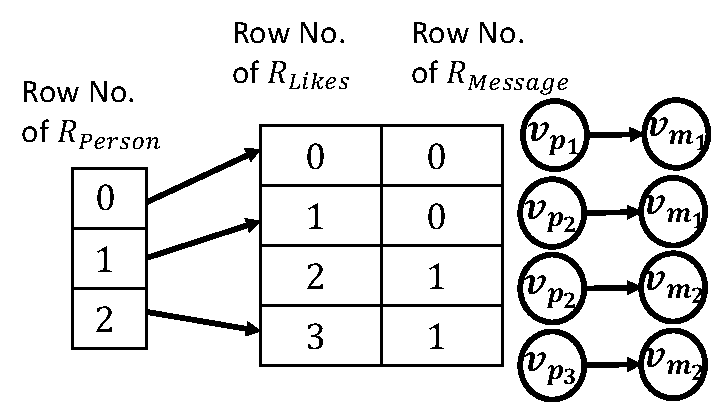
\includegraphics[width=.8\linewidth]{./figures/graph-index-likes.pdf}
    \caption{A graph index on edges labeled ``Likes'' on $G_1$ in \reffig{intro-rgmapping-example}.}
    \label{fig:graph-index}
\end{figure}

\subsubsection{Graph Index}
\label{sec:graph-index}

In a property graph, the adjacency relationships between vertices and edges are obvious and the adjacent edges of a vertex can be obtained directly.
Moreover, a tuple in a relation corresponds to a vertex or an edge in the property graph according to the \rgmapping.
Therefore, by maintaining the relationships between vertices and edges via indices, the join operator can be markedly accelerated.
This improvement is achieved because for each tuple within a relation, the indices have pre-stored the tuples that are joinable with it.
As a result, it eliminates the necessity to iterate through every tuple of the counterpart relation, thereby enhancing the efficiency of the join process.
As this index structure mimics the adjacency relationship between vertices and edges, it is called a graph index.

Join operators that leverage graph indices are called predefined joins by GrainDB \cite{graindb}.
Specifically, an example of the graph index instantiated in GrainDB is shown in \reffig{graph-index}.
In detail, the graph index is built on edges labeled ``Likes'' in property graph $G_1$ of \reffig{intro-rgmapping-example}(a) and records the adjacency relationships of the vertices labeled ``Person'' and the edges labeled ``Likes''.
That is, according to the \rgmapping, for each tuple $t_p$ in $\relation{Person}$, the tuples in $\relation{Likes}$ that can be joined with $t_p$ can be directly obtained with the graph index and vice versa.

In detail, the graph index consists of two parts as shown in \reffig{graph-index}.
The first part in \reffig{graph-index}(a) is designed for efficiently accessing tuples in $\relation{Person}$ that can be joined with tuples in $\relation{Likes}$.
Specifically, a new column named ``pid\_rowid'' is added to $\relation{Person}$ and the new relation with more columns is called $\grelation{Person}$.
For each tuple $t \in \grelation{Person}$, $t.pid\_rowid$ is the row number of $t_p \in \relation{Person}$, where $t_p.person\_id = t.pid$.
Note that row numbers start from 0.
Take the first tuple in $\grelation{Likes}$ (denoted as $t_l$) as an example.
Because $t_l.pid = p_1$ and the tuple $t_p$ at row number 0 in $\relation{Person}$ satisfies $t_p.person\_id = p_1 = t_l.pid$, we have $t_l.pid\_rowid = 0$.
With this graph index, given a tuple $t$ in $\grelation{Likes}$, the tuple in $\relation{Person}$ that are joinable with $t$ can be retrieved without scanning $\relation{Person}$.

However, given a tuple $t_p$ in $\relation{Person}$, we cannot leverage the graph index in \reffig{graph-index}(a) to directly access tuples in $\grelation{Likes}$ joinable with $t_p$, because it is unknown which rows of $\grelation{Likes}$ contain $pid$ values equal to $t_p.person\_id$.
Therefore, the adjacency list in \reffig{graph-index}(b) is constructed to solve this problem.
To elaborate, the first column contains the row numbers in $\relation{Person}$.
For example, row number 1 represents the second tuple in $\relation{Person}$ with $person\_id = p_2$ (denoted by $t_{p_2}$) and this tuple corresponds to $v_{p_2}$ in $G_1$.
The second column records the row numbers in $\grelation{Likes}$.
With this column, the edges adjacent to a given vertex can be retrieved efficiently.
For example, the edges adjacent to $v_{p_2}$ (i.e., $e_{l_2}$ and $e_{l_3}$ in $G_1$) are stored at row 1 and row 2 of $\grelation{Likes}$.
It means that the second and third tuples in $\grelation{Likes}$ can be joined with $t_{p_2}$.

If the adjacent relationships between vertices labeled ``Message'' and edges labeled ``Likes'' are also recorded in this index, the third column in \reffig{graph-index} is added.
With this column, the neighbors of given vertices can be quickly accessed.
It means that given a tuple $t_p$ in $\relation{Person}$, let $T_{Likes}$ be the set of tuples in $\relation{Likes}$ which can be joined with $t_p$, and then the tuples in $\relation{Message}$ which can be joined with a tuple in $\relation{Likes}$ can be quickly obtained.
For example, the neighbors connected to $v_{p_2}$, connected through edges labeled ``Likes'', include $v_{m_1}$ and $v_{m_2}$, whose corresponding tuples are at row 0 and row 1 in $\relation{Message}$.
This information can be quickly ascertained through the graph index.

\subsubsection{Physical Implementation}
\label{sec:join-matching-operator}
In implementing a logical matching plans, the inputs of join operators are two relations, i.e., $R_1 \Join R_2$, where $\theta$ is the join condition.
The join operators can be divided into three categories based on $R_2$.

Firstly, if $R_2$ is not obtained by a matching operator, then the join operator is implemented with
\begin{equation*}
    R_1 \Join R_2.
\end{equation*}

Secondly, if $R_2$ is obtained by a matching operator whose pattern graph is an edge, then the join operator is implemented as an \expandvertex~operator.
Specifically, denote the matching operator by $\matching(\pattern_e)$, where $\pattern_e$ consists of two vertices $u_s, u_t$ and an edge $e$ connecting them.
Let $\lambda^s_e$ and $\lambda^t_e$ be functions that associate tuples in $\relation{\vlabel{(e)}}$ with those in $\relation{\vlabel(u_s)}$ and $\relation{\vlabel(u_t)}$, respectively.
Then, the $\expandvertex(R_1, \pattern_e)$ is implemented with
\begin{equation*}
    R_1 \Join (\relation{\vlabel{(u_s)}} \Join_{\lambda^{s}_{e}} \relation{\vlabel{(e)}} \Join_{\lambda^{t}_{e}} \relation{\vlabel{(u_t)}}).
\end{equation*}
If graph indices have been built on $\relation{\mathcal{L}(e)}$, the joins between $\relation{\mathcal{L}(u_s)}$, $\relation{\mathcal{L}(e)}$, and $\relation{\mathcal{L}(u_t)}$ can be implemented more efficiently by leveraging the graph indices.
Moreover, if there is no need to retain attributes on $e$ and there are no constraints on $e$, graph indices can be applied to get neighbors of $u_s$ directly without scanning $\relation{\mathcal{L}(e)}$.

Thirdly, if $R_2$ is obtained by a matching operator whose pattern graph is a complete star, then the join operator is implemented as an \expandintersect~operator.
Before the \expandintersect~operator is defined, we first propose the $\intersect(alist, rlist)$~operator.
Specifically, the \intersect~operator takes a list of attribute names $alist$ and a list of relations $rlist = \{\relation{1}, \cdots, \relation{m}\}$ as inputs.
Attributes in $alist$ are shared by relations in $rlist$.
Let $t_1, \cdots, t_k$ be tuples in $\relation{1}, \cdots, \relation{m}$, respectively.
These tuples are joined together if and only if they have the same values on attributes in $alist$.


Denote the matching operator by $\matching(\pattern_s)$, where $\pattern_s = (v_r; \mathcal{H})$ and $\mathcal{H} = \{v_1, \cdots, v_k\}, k \geq 2$.
Let $e_1, \cdots, e_k$ be the edges connecting $v_1, \cdots, v_k$ and $v_r$, respectively.
Moreover, we have $\lambda^s_{e_i}$ and $\lambda^t_{e_i}$ mapping tuples from $\relation{\lab(e_i)}$ to $\relation{\lab(v_i)}$, and from $\relation{\lab(e_i)}$ to $\relation{\lab(v_r)}$, respectively.
Then, the $\expandintersect$($\relation{1}$, $\pattern_s$)~operator is implemented as
\begin{equation*}
    \intersect(\{v_r\}, \{\expandvertex(R_1, \pattern_{v_1}), \cdots, \expandvertex(R_1, \pattern_{v_k})\}),
\end{equation*}
where $\pattern_{v_i}$ represents a pattern with an edge connecting $v_i$ and $v_r$.

\begin{example}
    Given the pattern graph $\pattern$ shown in \reffig{intro-rgmapping-example}(b), a possible physical implementation for $\matching(\pattern)$ is as follows:
    \begin{equation*}
        \expandintersect(\expandvertex(\relation{\lab(u_{p_1})}, \pattern_{0}), \pattern_{s}),
    \end{equation*}
    where $\pattern_{0}$ consists of an edge connecting $u_{p_1}$ and $u_{p_2}$, while $\pattern_{s}$ is a complete star with $v_r = u_m$ and $\mathcal{H} = \{u_{p_1}, u_{p_2}\}$.
\end{example}
